\def\UseMinted{}
\documentclass[../main.tex]{subfiles}
\begin{document}
	
	
\section{Rozwiązanie -- koncepcja}
Celem jest przesył wiadomości ASANa do SIMICSa.

\paragraph{Ogólny zamysł}
\begin{itemize}
	\item SIMICS utworzy dodatkowy region pamięci, który posłuży jako bufor do
		komunikacji. ASAN będzie tam wpisywał informacje, a SIMICS czytał.
	\item ASAN nie potrafi printować do osobnego pliku, logu, ani niczego
		podobnego. Musimy więc mieć sposób na odfiltrowanie jego wiadomości od
		pozostałych "śmieci", które potencjalnie może printować testowany
		program. W tym celu nadpiszemy jedną z funkcji w
		\mintinline{sh}{libasan.so}, która jest wywoływana w momencie
		printowania przez ASANa, i wstrzykniemy tam kod, który będzie pisał do
		regionu pamięci SIMICSa.
	\item SIMICS musi wiedzieć, kiedy powinien odczytać coś z pamięci i
		potraktować jako wiadomość. W tym celu użyjemy jego funkcji "MAGIC
		instructions". Nasz kod wstrzyknięty w ASANa skorzysta z MAGIC aby
		wysyłać powiadomienia do SIMICSa.
\end{itemize}

\paragraph{Szczegóły}
\begin{itemize}
	\item W przypadku Linuxa, potrzebna jest modyfikacja device tree, aby
		zawiadomić jądro o istnieniu dodatkowego regionu pamięci.
	\item Jeśli nasz testowany program przebywa w userspace, nie jest możliwe
		bezpośrednie pisanie do regionu pamięci. Konieczne jest napisanie
		modułu, który umożliwi interakcję z tym regionem. W naszym przypadku
		mamy moduł, który wystawia proste urządzenie znakowe.
	\item W SIMICSie, konieczne będzie napisanie hooka, który nasłuchuje MAGIC
		instructions i odczytuje pamięć.
\end{itemize}


\section{Rozwiązanie -- implementacja}
Nasze rozwiązanie obejmuje platformę symulacyjną \mintinline{sh}{risc-v-simple} w SIMICS z systemem Linux oraz programem skompilowanym z sanitizerem. Do programu celowo wprowadziliśmy błędny dostęp do pamięci:

\begin{listing}[H]
	\begin{minted}[highlightlines={5}]{c}
		/* program: bad.c */
		int main(int argc, char **argv)
		{
			volatile int a[5] = {0};
			a[6] = argc;
			return 0;
		}
	\end{minted}
\end{listing}

\subsection{Linux}

\subsubsection{Sterownik}
Napisaliśmy prosty sterownik (moduł jądra Linux) do obsługi bufora na wyjście sanitizera. Moduł ten pozwala nam na wpisywanie ciągów znaków do zdefiniowanego przez nas obszaru pamięci w celu ich późniejszego odczytania przez emulator SIMICS.


\subsubsection{External Buildroot Toolchain}
Stworzyliśmy external toolchain w Buildroot w celu budowania naszego modułu dla jądra Linuxa wraz z obrazem systemu. Nasz system dla SIMICSa jest zdefiniowany następującym defconfigiem:

\begin{listing}[H]
	\begin{minted}[highlightlines={}]{txt}
# Architecture
BR2_riscv=y
BR2_RISCV_64=y

# Kernel
BR2_LINUX_KERNEL=y
BR2_LINUX_KERNEL_USE_ARCH_DEFAULT_CONFIG=y
BR2_LINUX_KERNEL_CUSTOM_VERSION_VALUE="5.17"
BR2_PACKAGE_HOST_LINUX_HEADERS_CUSTOM_5_17=y
BR2_LINUX_KERNEL_IMAGE=y

# Boot loader
BR2_TARGET_OPENSBI=y
BR2_TARGET_OPENSBI_PLAT="generic"

# Root file system
BR2_TARGET_ROOTFS_EXT2=y

# Host packages
BR2_PACKAGE_HOST_DTC=y
		\end{minted}
	\end{listing}

\subsubsection{Modyfikacja Device-Tree}
	Do drzewa urządzeń dodaliśmy własne urządzenie (simics\_shm), które jest buforem pamięci.
	Adres 0x20000000 został dobrany ręcznie pod platformę SIMICSa, na której się opieraliśmy
	(brak kolizji z innymi regionami pamięci). Rozmiar 0x4000 odpowiada 4\,KiB i został uznany
	jako wystarczająco duży, by pomieścić printy ASANa (największe, które zaobserwowaliśmy,
	miały około 1\,KiB).
	\begin{listing}[H]
		\begin{minted}[highlightlines={}]{sh}
simics_shm: simics_shm@20000000 {
	compatible = "simics_shm";
	device_type = "memory";
	reg = <0x00 0x20000000 0x00 0x4000>;
	status = "open";
};
		\end{minted}
	\end{listing}
	\noindent
	Następnie zmodyfikowane drzewo urządzeń budujemy do postaci binarnej, poleceniem
	
	\begin{listing}[H]
		\begin{minted}[highlightlines={}]{sh}
dtc -O dtb -o risc-v-simple.dtb risc-v-simple.dts
		\end{minted}
	\end{listing}


\subsubsection{Overlay dla Buildroot}
Overlay w Buildroot do dołączania programów lub plików do platformy docelowej do systemu plików. Wydał nam się najszybszym sposobem na statyczne osadzenie naszego programu w systemie. Głównie dlatego, że go już znaliśmy.

\subsubsection{Budowanie systemu}
Budowaliśmy system Linux, jak już wcześniej wspomniano korzystając z Buildroota i dodając mu odpowiednie flagi służące do obsługi externala oraz overlay'a.

\subsubsection{Dodawanie systemu do SIMICS}
Wgranie zbudowanego systemu do platformy emulowanej można wykonać poprzez (i tak to zrobiliśmy) linkowanie plików wynikowych z budowania systemów w Buildroot do folderu targets w platformie risc-v-simple w SIMICS, wykonaliśmy to poleceniem:
	\begin{listing}[H]
		\begin{minted}[highlightlines={}]{sh}
ln -r -s ~/buildroot/output/images/* \
         ~/simics/simics-risc-v-simple-7.x.x/...
         ...targets/risc-v-simple/images/linux/
		\end{minted}
	\end{listing}
\noindent
Dzięki temu nasza platforma po przebudowaniu będzie widoczna w aktualnej wersji z poziomu SIMICS, bez potrzeby ponownego kopiowania plików.



\subsection{SIMICS (i jego konfiguracja)}
\subsubsection{Dodawanie urządzenia}
Aby dodać urządzenie w emulatorze, aby adresy pamięci podane w naszym sterowniku były poprawnie intepretowane przez SIMICS i jądro Linuxa, stworzylismy każdorazowo obiekt:
	\begin{listing}[H]
		\begin{minted}[highlightlines={}]{simics}
fb_img = simics.SIM_create_object(
	"ram", f"{fb_ns}.buffer", image=None,
	self_allocated_image_size=size_bytes)
		\end{minted}
	\end{listing}
\subsubsection{Skrypt inicjujący platformę}
Aby nie podawać za każdym razem kilku komend związanych z utworzeniem obiektu naszej pamięci oraz ładowania platformy, napisaliśmy skrypt:
	\begin{listing}[H]
	\begin{minted}[highlightlines={}]{sh}
load-target "risc-v-simple/linux"
@SIM_create_object("ram","board.sanitizer_shm",
                   image=None, self_allocated_image_size=0x1000)
board.phys_mem.add-map board.sanitizer_shm 0x20000000 0x1000
	\end{minted}
\end{listing}

\subsubsection{Python MAGIC hook}
Napisaliśmy też skrypt w języku python do uruchamiania w SIMICS, aby przechwtywać MAGIC instructions.
Konwencjonalnie przyjęliśmy, że naszym \mintinline{c}{MAGIC_NUMBER} będzie \mintinline{c}{28}.
	\begin{listing}[H]
	\begin{minted}[highlightlines={}]{sh}
def branch():
	while True:
		conf.bp.magic.cli_cmds.wait_for(number=MAGIC_NUMBER)
		print("asan: ", end="")
		addr = SANITIZER_SHM_ADDR
		while True:
			byte = conf.board.phys_mem.memory[addr]
			if byte == 0:
				break
			print(chr(byte), end="")
			if byte == 10:
				print("asan: ", end="")
			addr += 1
		print()
	\end{minted}
\end{listing}

\subsection{Kompilacja programu}

ASAN wywołuje wewnętrznie funkcję \mintinline{c}{__sanitizer_on_print()} za
każdym razem, kiedy printuje informację dotyczącą błędów pamięciowych. Aby
nadpisać tę funkcję, definiujemy ją po swojemu w
\mintinline{sh}{libsan-overlay.c}:

	\begin{listing}[H]
	\begin{minted}[highlightlines={}]{c}
/* biblioteka: libsan-overlay.c */
#include <magic-instruction.h>  /* Nagłówek SIMICSa */

#define SIMICS_SHM_FPATH "/dev/simics_shm"
#define MAGIC_NUMBER 28

void __sanitizer_on_print(const char *str)
{
	/* Wersja skrócona */
	FILE *file;
	file = fopen(SIMICS_SHM_FPATH, "w");
	fwrite(str, sizeof(*str), str_len, file);
	MAGIC(MAGIC_NUMBER);
}
	\end{minted}
\end{listing}
\noindent
Nasza wersja funkcji otwiera wpisuje \mintinline{c}{str} do urządzenia
znakowego, które tworzy simics\_shm, a następnie emituje MAGIC instruction,
dając SIMICSowi znak, że może odczytać zawartość.

\paragraph{Trik obiektowy} Aby nadpisać funkcję bez ingerencji w kod źródłowy
testowanego programu, kompilujemy testowany program do pliku obiektowego,
kompilujemy \mintinline{sh}{libsan-overlay} do pliku obiektowego, następnie
łączymy dwa pliki obiektowe w jeden, i dopiero ten wynikowy linkujemy z ASANem:

	\begin{listing}[H]
	\begin{minted}[highlightlines={}]{sh}
# Komendy uproszczone, żeby się mieściły
CC -c -Isimics/.../include/simics/ libsan-overlay.c
CC -c -g -Og -static-libasan -fsanitize=address bad.c
LD -o combined.o -r bad.o libsan-overlay.o
CC -o bad combined.o -static-libasan -fsanitize=address
	\end{minted}
\end{listing}
\noindent
Dzięki tej kolejności, uniemożliwiamy ASANowi zdefiniowanie swojej wersji \\
\mintinline{c}{__sanitizer_on_print()}, ponieważ byłoby to powieleniem symbolu.

\subsection{Uruchomienie platformy (demonstracja działania)}

\begin{enumerate}
	\item Budowanie systemu
	\item Budowanie aplikacji z sanitizerem (\mintinline{sh}{make})
	
	\item Uruchomienie SIMICS, a w emulatorze:
	\begin{enumerate}
		\item Ładujemy platformę (\mintinline{sh}{run-script map_memory.simics})
		\item Uruchamiamy system (\mintinline{sh}{run})
		\item Uruchamiamy skrypt Python (\mintinline{sh}{run-script magic-hook.py})
		\item Tworzymy urządzenie znakowe (\mintinline{sh}{modprobe simics_shm})
		\item Uruchamiany program (\mintinline{sh}{./bad})
		\item Obserwujemy wyniki:
			\begin{figure}
				\centering
				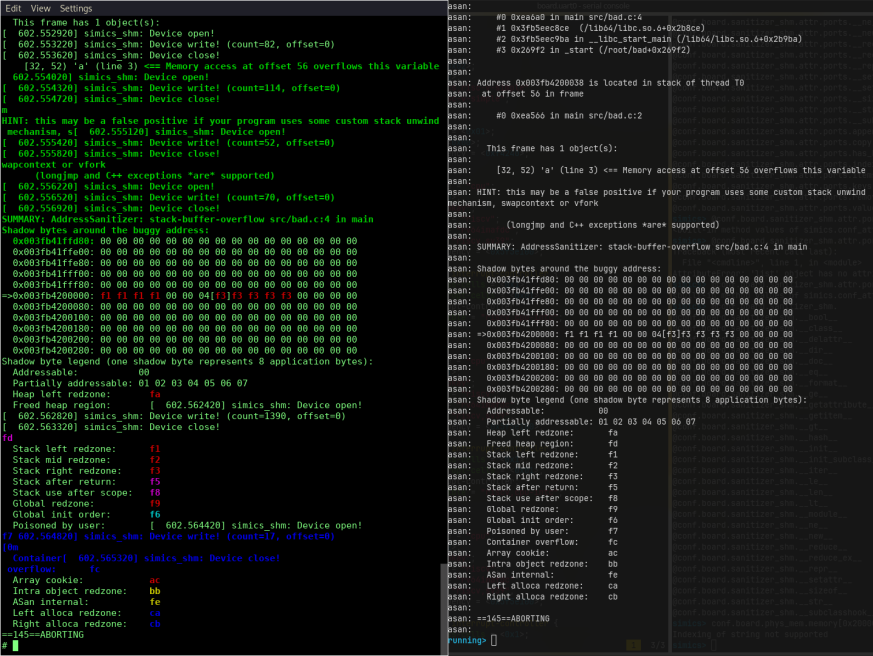
\includegraphics[width=0.8\linewidth]{images/end}
				\caption{Końcowy rezultat projektu - uruchomiony SIMICS, w nim Linux i nasz program z sanitizerem. Widać, że print sanitizera udało się przenieść do terminala z emulatorem}
				\label{fig:end}
			\end{figure}
	\end{enumerate}
\end{enumerate}


\end{document}
